\documentclass[10pt, aspectratio=169]{beamer}

%\usepackage[top = 1 in, bottom = 1 in, left = 1 in, right = 1 in]{geometry}

\usepackage{amsmath}
\allowdisplaybreaks[1]
\usepackage{amssymb, amsfonts}
\usepackage{enumerate}
\usepackage{multirow}
\usepackage{hhline}
\usepackage{array}
\usepackage{longtable}
\usepackage{graphicx}
\usepackage{tabularray}
\usepackage{undertilde}
\usepackage{dingbat}
\usepackage{fontawesome5}
\usepackage{tasks}
\usepackage{bbding}
\usepackage{twemojis}
% how to use bull's eye ----- \scalebox{2.0}{\twemoji{bullseye}}
\usepackage{customdice}
% how to put dice face ------ \dice{2}
\usepackage{pgfplots}
\pgfplotsset{compat=1.17}

\usepackage{fontspec}
\setmainfont{Century Schoolbook}
\renewcommand{\familydefault}{\rmdefault}

\usepackage{unicode-math}
\setmathfont{Latin Modern Math}

\usetheme{Warsaw}
\setbeamertemplate{headline}{}
\setbeamertemplate{footline}[page number in head/foot]{}
\usecolortheme{default}

\setbeamercolor{block title}{fg=blue!80!black, bg=blue!20}
\setbeamercolor{block body}{fg=black, bg=blue!5}

\usetikzlibrary{overlay-beamer-styles}

\title{Exponential Distribution as a Lifetime Model}
\author{Barsha$-$Arnab$-$Ritik$-$Rudransh$-$Sayan$-$Sujil$-$Ananda}
\date{}


\begin{document}


\begin{frame}
	\titlepage
\end{frame}

\begin{frame}{Contents}
    \tableofcontents
\end{frame}


\section{Introduction}

\begin{frame}{Introduction}
\onslide<1->{Lifetime data / survival time data measure the \underline{time to a certain event}, such as failure, death etc. These times are subject to random variations, and like any random variables, form a \underline{probability distribution}.} \\[1em]

\onslide<2->{Time$(T)$ is a non-negative continuous $(T \geq 0)$ quantity and one of the simplest distributions to model lifetime data is the \underline{Exponential Distribution}.}
\end{frame}

\begin{frame}{Introduction}
\onslide<1->{The distribution of survival times is usually characterized by 3 functions as follows :}
\begin{itemize}
\item<2-> the Probability Density Function
\item<3-> the Survival Function
\item<4-> the Hazard Function
\end{itemize}

\vspace{0.5cm}

\onslide<5->{\dice{4} \hspace{0.1cm} the Cumulative Hazard Function}
\end{frame}

\section{Probability Density Function}

\begin{frame}{Probability Density Function}
If the lifetime $T$  follows the exponential distribution with \underline{rate $\lambda \in \mathbb{R^{+}}$}, the probability density function $f : (-\infty, \infty) \rightarrow [0, \infty)$ is given by

\begin{equation*}
	 f(t) =
		\begin{cases}
		 \lambda e^{-\lambda t}, & t > 0  \\
		 0, & \text{otherwise}.
		\end{cases}
\end{equation*}
\end{frame}


\begin{frame}{Exponential PDF and CDF}

\begin{columns}
\begin{column}{0.49\textwidth}
\centering
\begin{tikzpicture}
\begin{axis}[
    width=\textwidth,
    height=5cm,
    domain=0:5,
    samples=100,
    xlabel={$t$}, ylabel={$f(t)$},
    ymin=0, ymax=2.5,
    axis lines=left,
    grid=both,
    legend style={at={(0.95,0.95)}, anchor=north east},
]

\only<1->{%
    \addplot[blue, thick] {0.5*exp(-0.5*x)};
    \addlegendentry{$\lambda = 0.5$}
}

\only<2->{%
    \addplot[red, thick] {1.0*exp(-1.0*x)};
    \addlegendentry{$\lambda = 1.0$}
}

\only<3->{%
    \addplot[green, thick] {1.5*exp(-1.5*x)};
    \addlegendentry{$\lambda = 1.5$}
}

\only<4->{%
    \addplot[magenta, thick] {2.0*exp(-2.0*x)};
    \addlegendentry{$\lambda = 2.0$}
}

\end{axis}
\end{tikzpicture}
\end{column}

\begin{column}{0.49\textwidth}
\centering
\begin{tikzpicture}
\begin{axis}[
    width=\textwidth,
    height=5cm,
    domain=0:5,
    samples=100,
    xlabel={$t$}, ylabel={$F(t)$},
    ymin=0, ymax=1.05,
    axis lines=left,
    grid=both,
    legend style={at={(0.95,0.95)}, anchor=north east},
]

\only<1->{%
    \addplot[blue, thick] {1 - exp(-0.5*x)};
    \addlegendentry{$\lambda = 0.5$}
}

\only<2->{%
    \addplot[red, thick] {1 - exp(-1.0*x)};
    \addlegendentry{$\lambda = 1.0$}
}

\only<3->{%
    \addplot[green, thick] {1 - exp(-1.5*x)};
    \addlegendentry{$\lambda = 1.5$}
}

\only<4->{%
    \addplot[magenta, thick] {1 - exp(-2*x)};
    \addlegendentry{$\lambda = 2.0$}
}

\end{axis}
\end{tikzpicture}
\end{column}
\end{columns}

\end{frame}



\section{Survival Function}

\begin{frame}{Survival Function}

\onslide<1->{From definition, with $F(\cdot)$ being the CDF of $T$, Survival function $S : [0, \infty) \rightarrow [0, 1]$ is given by $$S(t) = P[T > t] = 1 - F(t) \,\, \forall t \geq 0.$$} \\[0.5em]

\onslide<2->{We calculate}
\begin{align*}
\onslide<3->{\forall t \geq 0, \,\, F(t) &= \int \limits_{0}^{t} f(x) dx} \\
\onslide<4->{&= \int \limits_{0}^{t} \lambda e^{-\lambda x} dx = \lambda \left[-\dfrac{e^{-\lambda x}}{\lambda}\right]_{0}^{t} \\
&= 1 - e^{-\lambda t}}
\end{align*}

\begin{itemize}
\item<5-> $S(t) = e^{-\lambda t} \,\, \forall t \geq 0$
\end{itemize}

\end{frame}

\begin{frame}{Exponential CDF and Survival Function}
\begin{tikzpicture}
 \begin{axis}[
    width=10cm,
    height=7cm,
    domain=0:5,
    samples=100,
    xlabel={$t$},
    ylabel={$F(t),S(t)$},
    ymin=0, ymax=1,
    axis lines=left,
    grid=both,
    legend style={at={(0.95,0.95)}, anchor=north east}
]

\only<1->{%
    \addplot[blue, dashed] {1-exp(-0.5*x)};
	\addlegendentry{$F(t), \lambda = 0.5$}

}

\only<2->{%
    \addplot[blue, thick] {exp(-0.5*x)};
    \addlegendentry{$S(t), \lambda = 0.5$}
}
    
\only<3->{%
    \addplot[red, dashed] {1-exp(-2.0*x)};
	\addlegendentry{$F(t), \lambda = 2.0$}

}

\only<4->{%
    \addplot[red, thick] {exp(-2.0*x)};
    \addlegendentry{$S(t), \lambda = 2.0$}
}
\end{axis}
\end{tikzpicture}
\end{frame}


\begin{frame}{Exponential Survival Function}
\begin{tikzpicture}
 \begin{axis}[
    width=10cm,
    height=7cm,
    domain=0:5,
    samples=100,
    xlabel={$t$},
    ylabel={$S(t)$},
    ymin=0, ymax=1,
    axis lines=left,
    grid=both,
    legend style={at={(0.95,0.95)}, anchor=north east}
]

\only<1->{%
    \addplot[blue, thick] {exp(-0.5*x)};
    \addlegendentry{$\lambda = 0.5$}
}

\only<2->{%
    \addplot[red, thick] {exp(-1.0*x)};
    \addlegendentry{$\lambda = 1.0$}
}

\only<3->{%
    \addplot[green, thick] {exp(-1.5*x)};
    \addlegendentry{$\lambda = 1.5$}
}

\only<4->{%
    \addplot[magenta, thick] {exp(-2.5*x)};
    \addlegendentry{$\lambda = 2.5$}
}
\end{axis}
\end{tikzpicture}
\end{frame}

\section{Hazard Function}

\begin{frame}{Hazard Function}
\onslide<1->{The Hazard function $h : [0, \infty) \rightarrow [0, \infty)$ is defined as
\[
h(t) = \lim \limits_{\Delta t \to 0} \dfrac{
   P\left[
    \begin{array}{c}
      \text{an individual fails in the time interval } (t, t + \Delta t) \\
      \text{given the individual has survived to } t
    \end{array}
  \right]
}{
  \Delta t
}
\,\, \forall t \geq 0.
\]}

\onslide<2->{A simple derivation leads to $$h(t) = \dfrac{f(t)}{S(t)} \,\, \forall t \geq 0.$$}
\end{frame}

\begin{frame}{Hazard Function}
We have
\begin{itemize}
\item<1-> $f(t) = \lambda e^{-\lambda t} \cdot I_{(0, \infty)}(t), \,\, \lambda > 0$.
\item<2-> $S(t) = e^{-\lambda t} \,\, \forall t \geq 0$.
\end{itemize}

\vspace{0.5cm}

\onslide<3->{\leftpointright \hspace{0.1cm} $h(t) = \lambda \,\, \forall t \geq 0$, a constant, independent of $t$.}

\vspace{0.5cm}

\onslide<4->{\smallpencil \hspace{0.1cm} A constant hazard rate is a \underline{necessary and sufficient} condition for a continuous lifetime distribution to be exponential.}
\end{frame}

\begin{frame}
\begin{tikzpicture}
 \begin{axis}[
    width=10cm,
    height=7cm,
    domain=0:5,
    samples=100,
    xlabel={$t$},
    ylabel={$h(t)$},
    ymin=0, ymax=2.5,
    axis lines=left,
    grid=both,
    legend style={at={(0.95,0.95)}, anchor=north east}
]

\only<1->{%
    \addplot[blue, thick] {0.5};
    \addlegendentry{$\lambda = 0.5$}
}

\only<2->{%
    \addplot[red, thick] {1.0};
    \addlegendentry{$\lambda = 1.0$}
}

\only<3->{%
    \addplot[green, thick] {1.5};
    \addlegendentry{$\lambda = 1.5$}
}

\only<4->{%
    \addplot[magenta, thick] {2};
    \addlegendentry{$\lambda = 2$}
}
\end{axis}
\end{tikzpicture}
\end{frame}

\section{Cumulative Hazard Function}

\begin{frame}{Cumulative Hazard Function}
\onslide<1->{The Cumulative Hazard Function $H : [0, \infty) \rightarrow [0, \infty)$ is defined by $$H(t) = \int \limits_{0}^{t} h(x) dx.$$} \\[1em]

\onslide<2->{For $T \sim \text{Exp}(\text{rate} = \lambda)$, $$H(t) = \lambda t \,\, \forall t \geq 0.$$}
\end{frame}

\begin{frame}
\begin{tikzpicture}
 \begin{axis}[
    width=10cm,
    height=7cm,
    domain=0:5,
    samples=100,
    xlabel={$t$},
    ylabel={$H(t)$},
    ymin=0, ymax=2,
    axis lines=left,
    grid=both,
    legend style={at={(0.95,0.95)}, anchor=north east}
]

\only<1->{%
    \addplot[blue, thick] {0.5*x};
    \addlegendentry{$\lambda = 0.5$}
}

\only<2->{%
    \addplot[red, thick] {1.0*x};
    \addlegendentry{$\lambda = 1.0$}
}

\only<3->{%
    \addplot[green, thick] {1.5*x};
    \addlegendentry{$\lambda = 1.5$}
}

\only<4->{%
    \addplot[magenta, thick] {2*x};
    \addlegendentry{$\lambda = 2$}
}
\end{axis}
\end{tikzpicture}
\end{frame}

\end{document}